\chapter{\texorpdfstring{\MakeUppercase{Preston Royal Case Study}}{Preston Royal Case Study}}

Preston Royal Branch Library is a one-story building with
\SI{12400}{\feet\squared} of gross floor area. The library opened in 1954. The
facility consists of an open-space reading room and circulation, staff area,
and an auditorium.

The library is served by a single air handling unit. A BAS graphic of
the AHU is shown in \figref{} \ref{fig:PrestonRoyalAHUGraphic}. 

The AHU has 14 terminal units that serve the various areas of the
library and are shown in \figref{} \ref{fig:PrestonRoyalAHUGraphic} and
\ref{fig:PrestonRoyalTerminalUnitLayout}.

The terminal units are parallel fan powered boxes. A BAS graphic of one
of the terminal units is shown in \figref{}
\ref{fig:PrestonRoyalTerminalUnitGraphic}.

\begin{figure}
\centering
\includegraphics[width=\textwidth]{Images/PrestonRoyalAHUGraphic.PNG}
\caption{Preston Royal AHU BAS Graphic.}
\label{fig:PrestonRoyalAHUGraphic}
\end{figure}

\begin{figure}
\centering
\includegraphics[width=\textwidth]{Images/PrestonRoyalFPBLayoutGraphic.PNG}
\caption{Preston Royal terminal unit layout.}
\label{fig:PrestonRoyalTerminalUnitLayout}
\end{figure}

\begin{figure}
\centering
\includegraphics[width=\textwidth]{Images/PrestonRoyalTerminalUnitGraphic.PNG}
\caption{Preston Royal terminal unit graphic. }
\label{fig:PrestonRoyalTerminalUnitGraphic}
\end{figure}



\section{Preston Royal Zone Load Analysis}

The zone load profile for Preston Royal showed similarities to the NCTM
building. During operation, the estimated zone load fluctuated up and
down throughout the day. \figref{}
\ref{fig:2017-04-03-1250-ZoneLoadforFPB02-TikzData} shows an example of
how the zone load cycles up and down many times per hour. Again, the
hypothesized explanation for this is not that the actual heat gain in
the space is fluctuating, but that the HVAC controls are oscillating. 

\begin{figure}
\centering
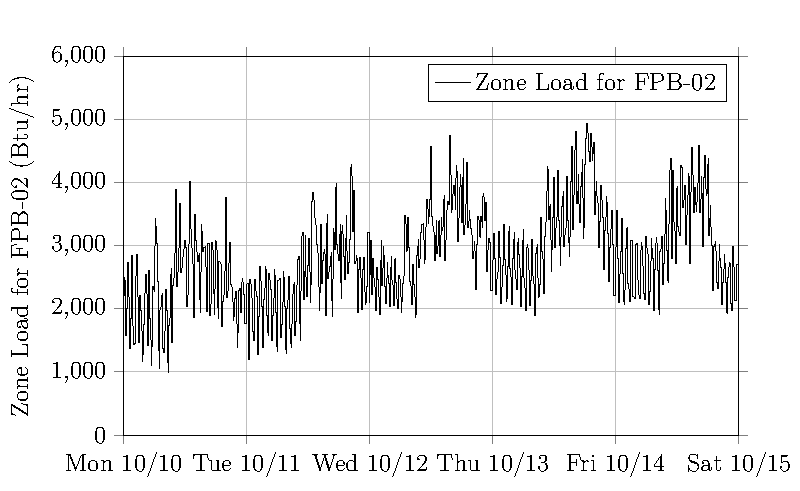
\includegraphics[]{Plots/2017-04-03-1250-ZoneLoadforFPB02-TikzData.pdf}
\caption{Zone load for FPB02 at Preston Royal Library.}
\label{fig:2017-04-03-1250-ZoneLoadforFPB02-TikzData}
\end{figure}


\figref{} \ref{fig:2017-06-05-0822-ZoneLoadforFPB02-TikzData} shows the
zone load for all the terminal units at Preston Royal Library for 3 days
from October 19\textsuperscript{th}, 2016 through October
21\textsuperscript{st}, 2016. Of interest to note is that within the
same space, one terminal unit can be experiencing a large cooling load
(FPB-11) while another terminal unit is calling for heating (FPB-08). 


\begin{figure}
\centering
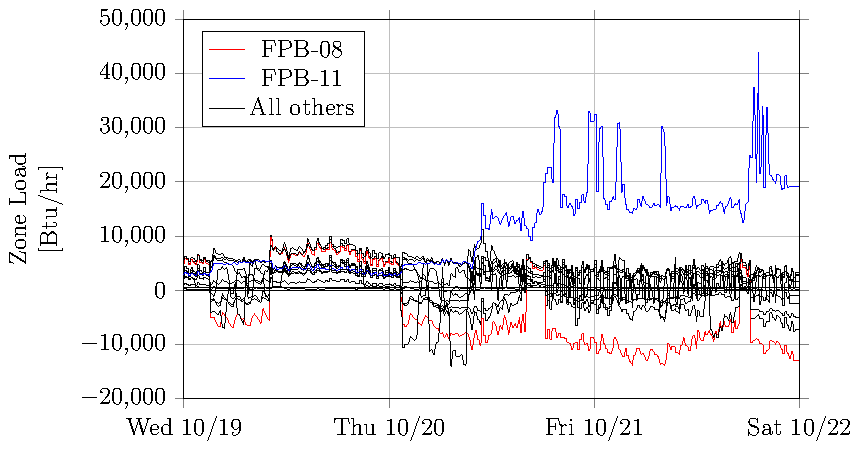
\includegraphics[]{Plots/2017-06-05-0822-ZoneLoadforFPB02-TikzData.pdf}
\caption{Zone load for all terminal units at Preston Royal Library.}
\label{fig:2017-06-05-0822-ZoneLoadforFPB02-TikzData}
\end{figure}

The optimization could not be completed for Preston Royal Library
because of data quality issues. The data was not produced consistently
and had long gaps during many days. In addition, a flow sensor for
FPB-05 was constant at 0, and this issue was not resolved. 


